\documentclass{beamer}
\usepackage[utf8]{inputenc}
\usepackage[T1]{fontenc}
\usepackage[frenchb]{babel}  
\usepackage{amssymb}
\usepackage{amsthm}
\usepackage{amsmath}
\usetheme{Warsaw}
\usepackage{graphicx}
\usepackage{ragged2e}

\addtobeamertemplate{navigation symbols}{}{%
	\usebeamerfont{footline}%
	\usebeamercolor[fg]{footline}%
	\hspace{1em}%
	\insertframenumber/\inserttotalframenumber
}
\title{Complexity of Neural Networks}
\author{Vasquez Alessandro}
\institute{Université Nice-Sophia-Antipolis}

\begin{document}

\frame{\titlepage}
\begin{frame}
\frametitle{Preliminaries}
\begin{columns}
	\begin{column}{0.47\textwidth}
		Neuron's representation:
		$y = \sigma (\sum_{j=1}^{n}w_jx_j - w_0)$ \\
		Transfer functions: 
		\begin{itemize}
			\item $   
			sign(t)  = 
			\begin{cases}
			0 &\quad\text{if } t \leq 0\\
			1 &\quad\text{if } t > 0 \\
			\end{cases}
			$
			\item $\sigma (t) = (1+e^{-t})^{-1}$
			%	\item $Pr(\sigma_T(t) = 1 ) = (1+e^{-t/T})^{-1} $
		\end{itemize}
	\end{column}
	\begin{column}{0.5\textwidth}
		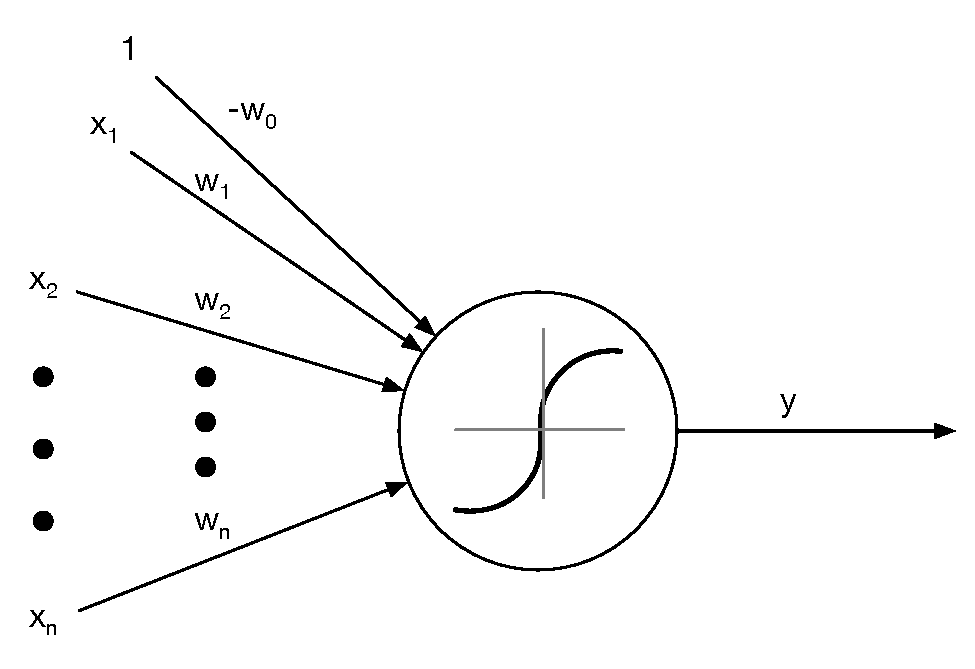
\includegraphics[width=1.1\textwidth]{images/neuron.eps}
	\end{column}
\end{columns}

\end{frame}


\begin{frame}
\frametitle{Preliminaries}
Neural nets can be
\begin{itemize}
	\item cyclic or acyclic
	\item symmetric or asymmetric w.r.t. interconnections
	\item continuous or discrete w.r.t. updates
	\item synchronous or asynchronous w.r.t. updates in discrete neural nets
\end{itemize}
\end{frame}


\begin{frame}
\frametitle{Preliminaries}
Type of neurons
\begin{itemize}
	\item perceptron (with transfer function)
	\item threshold gate (with binary valued-input)
	\item majority gate (all $w=1$, $b=\frac{|X|}{2}$)
\end{itemize}
\begin{definition}[Threshold function]
	\justify
	A boolean function $t: \{0,1\} \to \{0,1\} $ is a \textit{threshold function} if it is computable by a linear threshold unit.
\end{definition}
\end{frame}

\begin{frame}{Preliminaries}

Parameters for evaluating neural nets' complexity
\begin{itemize}
	\item size
	\item depth
	\item weight
\end{itemize}
We're going to consider discrete-weighted
\begin{itemize}
\item threshold gates-circuits
\item Hopfield nets
\end{itemize}
\end{frame}

\begin{frame}
\frametitle{Acyclic nets}
\framesubtitle{Weights and computational power}	
	\begin{theorem}
		\justify
		Any threshold function on $n$ variables can be computed by a threshold gate with integer weights $w_i$ st: $$|w_i| \leq \frac{(n+1)^{(n+1)/2}}{2^n}, \forall i =0,...,n.$$
	\end{theorem}
\end{frame}

\begin{frame}
\justify
\frametitle{Acyclic nets}
\framesubtitle{Weights and computational power}	
\begin{theorem}
	\justify
For infinitely many $n$, there are threshold functions on $n$ variables whose computation by a single threshold gate requires weights as large as $\frac{n^{n/2}}{2^n}.$
\end{theorem}
These theorems imply that there is a class of threshold gates of polynomially bounded weights. But even in the case of non-polynomially bounded weights, these can be represented in $O(s \log{s})$ bits.
\end{frame}

\begin{frame}
\justify
\frametitle{Circuit Classes}
\framesubtitle{Definitions}	
	\justify
	Let's consider acyclic networks which compute a boolean function $f: \{0,1\}^n \to \{0,1\}.$
	\begin{definition}[Complexity classes]
		\justify
		We define five class of functions computable by different classes of circuits.
		\begin{itemize}
			\item $NC^k: $ polynomial-size circuits of depth $ O(\log ^{k}(n)),$ using bounded fan-in AND, OR, and NOT gates,
			\item $AC^k: $ polynomial-size circuits of depth $ O(\log ^{k}(n)),$ using unbounded AND, OR, and NOT gates,
			\item $TC^k: $ threshold circuits of polynomial size and depth $O(log^k n),$
			\item $TC_d^0$ threshold circuits of polynomial size and depth $d,$
			\item $\widehat{TC}_d^0$ majority circuits of polynomial size and depth $d.$
		\end{itemize}
	\end{definition}
\end{frame}
\begin{frame}
\justify
	\frametitle{Circuit classes}
	\framesubtitle{Results}
	\begin{theorem}[Complexity classes' hierarchy]
		$$ AC^k \subseteq TC^k \subseteq NC^{k+1}. $$
		\[
			\widehat{TC}_d^0 \subseteq TC_d^0 \subseteq \widehat{TC}_{d+1}^0.
		\]
	\end{theorem}
We only know that $AC^0 \subset TC^0,$ e.g. because of the majority function, and $TC^0_1 \subset \widehat{TC^0_2}$ for the parity function.
\end{frame}

\begin{frame}
\frametitle{Acyclic nets}
\framesubtitle{Results}
The following problems are proved to be NP-complete.
\begin{definition}[Threshold circuit loading]
	\justify
	Given $\{(\vec{x_1}, b_1),...,(\vec{x_m}, b_m)\},$ where each $\vec{x_i} \in \{0,1\}^n$ and each $b_i \in \{0, 1\},$ and a directed acyclic graph, can we find a weight assignment st given $f$ the function computed by the resulting threshold circuit: $f(\vec{x_i})=b_i, \forall i = 1,...,m ?$
\end{definition}

\begin{definition}[Threshold circuit minimization]
	\justify
	Given $\{(\vec{x_1}, b_1),...,(\vec{x_m}, b_m)\},$ where each $\vec{x_i} \in \{0,1\}^n$ and each $b_i \in \{0, 1\},$ and $K \in \mathbb{N}$, does exists a threshold circuit of at most $K$ neurones st given $f$ the function computed by the resulting threshold circuit: $f(\vec{x_i})=b_i, \forall i = 1,...,m ?$
\end{definition}
\end{frame}

\begin{frame}
\frametitle{Cyclic nets}
\framesubtitle{Hopfield Networks}
\begin{definition}[Hopfield network]
Neural net in which
\begin{itemize}
	\item the weights $w_{ij}$ are symmetric
	\item the net has a vector $I$ which represents its global state
	\item each neuron $i$ has a local state $I_i$, where $I$ is the states' vector
	\item each neuron's state is updated asynchronously
	\item there's an "energy function" assigned to the network
\end{itemize}
\end{definition}
\end{frame}

\begin{frame}
	\frametitle{Hopfield Networks}
	The energy function is
	\[E=-\frac{1}{2}\sum_{i,j}w_{ij}s_is_j-\sum_iI_is_i \]
	If we derivate the energy function w.r.t. each $s_i$ and changing its sign we get
	\[
		\frac{\partial E}{\partial s_i} = I_i + \sum_{j}s_jw_{ij}, 
	\]
	for each neuron $i.$
\end{frame}

\begin{frame}{Hopfield Networks}
	If we consider the state of a neuron as its bias, we get
		\[
			\frac{\partial E}{\partial s_i} = b_i + \sum_{j}s_jw_{ij},
		\]
		which is the binary threshold decision rule computed locally by each neuron.
		In 1982 Hopfield proved that $E$ is a Lyapunov function. 
\end{frame}

\begin{frame}{Hopfield Network - Example}
	\includegraphics[width=.8\textwidth]{images/NN/Hopfieldnet.eps}
\end{frame}

\begin{frame}{Hopfield Network - Example}
\includegraphics[width=.8\textwidth]{images/NN/Hopfieldnet2.eps}
\end{frame}
\begin{frame}{Hopfield Network - Example}
\includegraphics[width=.8\textwidth]{images/NN/Hopfieldnet3.eps}
\end{frame}
\begin{frame}{Hopfield Network - Example}
\includegraphics[width=.8\textwidth]{images/NN/Hopfieldnet4.eps}
\end{frame}
\begin{frame}{Hopfield Network - Example}
\includegraphics[width=.8\textwidth]{images/NN/Hopfieldnet41.eps}
\end{frame}
\begin{frame}{Hopfield Network - Example}
\includegraphics[width=.8\textwidth]{images/NN/Hopfieldnet5.eps}
\end{frame}

\begin{frame}{Storage Rule}
\justify
	\begin{definition}[Storage Rule]
		\justify
		An algorithm which starts by a set of  vectors $\vec{X}=\{\vec{x_1},..,\vec{x_n}\}$ and builds an Hopfield net s.t. its stable state are those vector its called a \textit{storage rule.}
	\end{definition}
	Hopfield himself thought of its nets as an implementation of the \textit{associative memory}.
\end{frame}

\begin{frame}
\frametitle{Cyclic nets}
\framesubtitle{Results}
\begin{theorem}
	\justify
	In a symmetric Hopfield net with $w_{ij}$ integer weights and $n$ neurons, the convergence is obtain in 
	\[
	O(n^2 \cdot \max_{i,j} |w_{ij}|)
	\]
	asynchronous changes of neuron states.
\end{theorem}
\end{frame}

\begin{frame}
	\frametitle{Cyclic nets}
	\framesubtitle{Definitions}
	\begin{definition}[Attraction domain]
		\justify
		Let $\vec{x_i}$ be a stable global state for a given Hopfield net. The \textit{attraction domain} of $\vec{x_i}$ is the set of all vectors which are guaranteed to converge to $\vec{x_i}.$
	\end{definition}
	\begin{definition}[Attraction radius]
		\justify
		The \textit{attraction radius} of $x_i$ is the largest Hamming distance from which all other vectors are guaranteed to converge to $\vec{x_i}.$ The attraction radius determines the basin of attraction.
	\end{definition}
\end{frame}

\begin{frame}{Local vs global minimum}
\includegraphics[width=1\textwidth]{images/Energy_landscape.png}
	
\end{frame}

\begin{frame}{Oscillating synchronous update}
\includegraphics[width=.8\textwidth]{images/NN/Hopfieldnet6.eps}
\end{frame}

\begin{frame}
\frametitle{Cyclic nets}
\framesubtitle{NP-complete problems}
\justify
	\begin{itemize}
		\item Decide if a given symmetric, simple network has more than one stable state.
		\item Determine if a symmetric simple network converges to a given stable state from any other initial state.
	\end{itemize}
\end{frame}

\begin{frame}
\frametitle{Cyclic nets}
\framesubtitle{NP-hard problems}
\justify
\begin{itemize}
	\item Decide if a given asymmetric net under synchronous updates will converge from any (or all) initial state.
	\item Computing the attraction radius of a given stable state in a symmetric simple net.
\end{itemize}
\end{frame}

\begin{frame}
\frametitle{Open problems}
\begin{definition}[Hopfield Net Loading Problem]
	\justify
	Given a set of vectors $X=\{\vec{x_1}, .., \vec{x_m}\},$ where each $\vec{x_i} \in \{-1,1\}^n,$ and a constant $\rho,$ is there a symmetric net of $n$ neurons that has $X$ as stable states with attraction radii $\geq \rho?$
\end{definition}
\end{frame}

\begin{frame}
	\frametitle{Open problems}
The following questions are yet to be answered.
\begin{itemize}
	\item Is the Hopfield Net Loading Problem in $P$ or in $NP$?
	\item Are the separations $TC_d^0 \subseteq TC_{d+1}^0, \forall d\geq2$ proper ? 
	\item Does exist a $d$ s.t. $AC^0 \subseteq TC_d^0, $ i.e. does exists a class of $d-$depth majority circuits which can compute all functions computed by a depth 1, unbounded, AND-OR-NOT circuit ?
\end{itemize}
\end{frame}
\begin{frame}
\begin{center}
	Thank you for your attention.
\end{center}
\end{frame}

\end{document}
